
\chapter{Selected Plant Models} \label{chapter:models-used}

% Chapter introduction
For the reasons stated in Chapter \ref{chapter:exp-setup}, we conduct our experiments with \textit{in silico} plants.
This chapter starts with a set of formal requirements that plant simulations must meet for use in physical reservoir computing.
Then follows an overview of the FSPMs from the literature we have examined for use in this research.
Finally, we introduce the final selection of models and compare their traits and characteristics.


\section{Selection Criteria} \label{sec:model-selection-criteria}
% PRC requirements

Section \ref{fspm:selecting-models-for-rc} already formulated the general requirements of a plant model for use in the \acrshort{prc} framework.
This section now formalizes the search criteria from the point of view of the experiments we wish to conduct. 
The selected models must meet the following specifications:
% From the point of view of the experiments we wish to conduct, plant models must meet the following requirements:

\begin{enumerate}
    \item \textbf{Modeled as a dynamical system.} To observe reservoir dynamics, there must be a dynamical relationship between the structural elements of the plant.
    \item \textbf{Local observability of eco-physiological processes.} To create a readout of the reservoir, standard eco-physiological functions, such as surface temperature, transpiration rate, and stomatal conductance, must be observable at each of the discrete elements of the plant.
    \item \textbf{Sufficiently small simulation steps.} Small simulation steps can reveal dynamics that occur at shorter time scales. Ideally, we can observe dynamics at the second to hour scale.
    \item \textbf{(Pseudo-)static reservoir.} \acrlong{rc} assumes the reservoir dynamics are unchanging through time. To satisfy this condition, we limit our search to plant models l Research on the effect of plant growth on reservoir dynamics is out of scope for this research.
    \item \textbf{Practically observable physiological processes.} Section \ref{sec:considered-reservoirs} explained that there is a preference for models that simulate physiological processes which we can observe using existing (contactless) sensing technologies. 
\end{enumerate}

The first and second requirements are met by narrowing the search to functional-structural plant models, as was established in Chapter \ref{chapter:fspm}.
However, we must evaluate the third, fourth, and fifth conditions on a case-by-case basis.
For the fifth condition, Tables \ref{table:imaging-techniques} and \ref{table:non-imaging-techniques} can be used to determine which models to consider.


% Practical requirements
Some additional requirements arise from a practical aspect. 
First, the plant simulation must be able to run for a large number of time steps. 
This is needed to build a sufficiently large dataset to train readout models on. 
Also, observing fading memory effects requires a sufficient length of simulated steps.
Second, the model software must be easily adapted to extract the evolution of the reservoir state during simulation and store it in a time series dataset.


\section{Related Work} \label{sec:models-considered}

% Introduction to the list of models.
% We searched for FSPMs that fit our criteria through Quantitative Plant and a literature search
There are diverse models in the literature, but many do not meet all our demands.
There are a few common shortcomings.
For one, many FSPMs only model a limited set of physiological processes \citep{louarn_two_2020}.
These simulations are too narrow to gain convincing evidence of reservoir dynamics present in real-world plants.
Other published works show sophisticated architectures and solid real-world validations but do not make their simulations open source \citep{prieto_functionalstructural_2020}. 


% Discussion of considered of FSPMs.
Table \ref{table:models-related-work} shows a selection of plant models we examined more closely.
We briefly investigated V-Mango \citep{boudon_v-mango_2020} and WALTer \citep{lecarpentier_walter_2019}. Ultimately, we disregarded these models because they model growth with time steps of one day. 
This step size is too large to explore reservoir dynamics at the time scales we want to observe (\SI{1}{s}-\SI{1}{h}).

PlaNet-Maize \citep{lobet_modeling_2014} and Soybean FSPM \citep{coussement_turgor-driven_2020} are growth models, but the step size of one hour warrants taking a deeper look;
when the growth rate is very slow compared to the time scale of the target task, the reservoir can be regarded as approximately static, as \citet{pieters_reservoir_2022} demonstrated with \textit{in vivo} strawberry plants.
Unfortunately, we could not further explore this direction due to practical reasons.
PlaNet-Maize is open-source, but the code repository contains no documentation on getting started or making modifications.
The soybean model is closed-source but was made available to us by co-author T. De Swaef.
Regrettably, we met many difficulties setting up the simulation environment, and the GroIMP platform made it unintuitive to implement adaptations as an untrained user.
Because of these reasons, combined with the limited time scope of this project, we did not explore these models further.


\begin{table}[!ht]
    \raggedright
    \caption{\acrshort{fspm}s we explored for use in RC experiments. Models highlighted in bold are used for the final results presented in this work.}
    \def\arraystretch{1}%  1 is the default, change whatever you need
    \begin{tabular}{
        >{\raggedright} m{0.166\linewidth}
        >{\raggedright\arraybackslash} m{0.14\linewidth} 
        >{\centering\arraybackslash} m{0.1\linewidth}
        >{\centering\arraybackslash} m{0.11\linewidth}
        >{\raggedright\arraybackslash} m{0.166\linewidth}
        >{\centering\arraybackslash} m{0.13\linewidth}
    }
        \toprule
        \textbf{Model} & \textbf{Crop} & \textbf{Growth} & \textbf{Time Step} & \textbf{Implementation} & \textbf{Open Source} \\ 
        \midrule
        PlaNet-Maize \citep{lobet_modeling_2014} & Maize & Yes & \SI{1}{h} & Java & Yes \\
        \arrayrulecolor{black!10!white}
        \midrule
        \textbf{CN-Wheat \citep{barillot_cn-wheat_2016}} & \textbf{Common wheat} & \textbf{No} & \textbf{1 h} & \textbf{Python (OpenAlea)} & \textbf{Yes} \\
        \midrule
        \textbf{HydroShoot \citep{albasha_hydroshoot_2019}} & \textbf{Common grapevine} & \textbf{No} & \textbf{1 h} & \textbf{Python (OpenAlea)} & \textbf{Yes} \\
        \midrule
        WALTer \citep{lecarpentier_walter_2019} & Common wheat & Yes & \SI{1}{d} & Python (OpenAlea) & Yes \\
        \midrule
        Soybean FSPM \citep{coussement_turgor-driven_2020} & Soybean & Yes & \SI{1}{h} & Java (GroIMP) & No \\
        \midrule
        V-Mango \citep{boudon_v-mango_2020} & Mango tree & Yes & \SI{1}{d} & Python (OpenAlea), R & Yes \\
        \midrule
        WheatFspm \citep{gauthier_functional_2020} & Common wheat & Yes & \SI{1}{h} & Python (OpenAlea) & Yes \\ 
        \midrule
        \citet{prieto_functionalstructural_2020} (unnamed) & Common grapevine & No & \SI{1}{h} & Python (OpenAlea) & No \\
        \arrayrulecolor{black}
        \bottomrule
    \end{tabular}
    \label{table:models-related-work}
\end{table}

% Discussion of shortlisting of FSPMs.
HydroShoot \citep{albasha_hydroshoot_2019} and a similar, unnamed model by \citet{prieto_functionalstructural_2020} are both FSPMs of grapevine; they have a static geometry and model a diverse set of physiological functions involved in gas exchange.
As far as we could find, \citeauthor{prieto_functionalstructural_2020} did not publish the code for their model.
In contrast, HydroShoot is open source and very well documented.
It was straightforward to set up using the Conda package manager for Python. The use of well-documented libraries from the OpenAlea platform made it easy to track the plant's state or adjust its environment.

Finally, WheatFspm \citep{gauthier_functional_2020} is another growth model.
WheatFspm builds upon the prior work CN-Wheat \citep{barillot_cn-wheat_2016}, a post-vegetative growth model of the same species.
Because we prefer (pseudo-)static models, we used CN-Wheat for our experiments instead.
The simulation code provided in the source repository already extracts all physiological time series, making CN-Wheat a very convenient model for our purposes.

Both HydroShoot and CN-Wheat have a good overlap in the physiological processes and meteorological inputs they simulate. 
These shared qualities enable a closer comparison of how the models behave as reservoirs when solving the same regression tasks.
The following section introduces the two selected models in more detail and compares them from a \acrshort{rc} perspective.



\section{Selected Models} \label{sec:selected-models}

\subsection{HydroShoot}

% Overview
HydroShoot is an FSPM of \textit{Vitis vinifera}, otherwise known as the common grapevine.
It was published by \citet{albasha_hydroshoot_2019} as a study of the gas exchange of large plant canopies under water deficit conditions and to compare the effectiveness of different canopy shapes.
It is written in the Python programming language and is built on the OpenAlea platform.
 

% Functional architecture
HydroShoot consists of three main modules, simulating the water potential across structural segments, the energy budget of individual leaves, and transpiration and carbon assimilation of individual leaves.
Hydraulic pressure gradients across elements induce water flow, creating dynamical behavior between the elements.
The authors experimentally validated that gas exchange, leaf hydraulic pressure, and temperature are adequately simulated during daytime hours.
However, the model is prone to underestimate leaf temperature during nighttime hours.
Nonetheless, on the surface, HydroShoot appears to be a realistic simulation of plant dynamics and thus a good candidate for \acrshort{rc} research.


% Description of structural architecture
The model uses a static, predefined structure. 
The geometry is hand-modeled, based on measurements taken from real grapevine specimens.
Figure \ref{fig:hydroshoot-archi} shows an example of one of the canopy configurations modeled for HydroShoot.
Because HydroShoot does not simulate plant growth or tissue death, we should expect it to behave as an idealized static reservoir.
The entire structure consists of hundreds of elements, about three hundred of which are photosynthesizing leaves, depending on the 3D model.


% Model inputs
HydroShoot uses hourly meteorological inputs of solar incident shortwave irradiance (PAR), air temperature ($T_{\text{air}}$), relative humidity (RH), wind speed ($u$), CO$_2$ concentration, and atmospheric pressure ($P_a$).
However, in the simulations for the 2019 publication, the latter two are fixed to values of \SI{400}{ppm} and \SI{101.3}{kPa} respectively.


% Simulation details
The simulations in the original publication ran for four days with hourly time steps.
In correspondence with the authors, R. Albasha informed us that the model has been used in simulations up to one month in length, using \SI{2}{h} steps during the day and a \SI{12}{h} step for nighttime.
However, extending the simulation time requires modeling recurrent soil water potential over a longer time than is provided in the original simulation, which is out of scope for this work.
As a compromise, we ran the model in runs of 7 days with a simplified model of constant recurrent soil water potential (see \mbox{Appendix \ref{app:hydroshoot-sim-details}}).


\subsection{CN-Wheat}

% What is CN-Wheat?
CN-Wheat is a mechanistic model of \textit{Triticum aestivum}, more widely known as common wheat.
CN-Wheat was developed by \citet{barillot_cn-wheat_2016} and is also built on the OpenAlea platform.
The model was created to simulate carbon (C) and nitrogen (N) metabolism in wheat culms in the post-flowering stages of development.


% Breakdown of CN-Wheat's physiological model
The model simulates a rich set of eco-physiological processes that drive the C and N lifecycle inside the plant. 
This includes photosynthesis and transpiration, synthesis of CN metabolites, metabolite transport in phloem tissue, and interaction between metabolites and the root system.
The network of phloem tissue is simplified as a shared pool of C and N that facilitates communication between the functional-structural elements.
This simplified transport model limits flow dynamics to the gradients between the elements and this shared pool of resources.
It reduces the potential for more intricate dynamics within the network, such as the local influence of neighboring elements over each other's behavior.


% Breakdown of CN-Wheat's structural architecture
Figure \ref{fig:cnwheat-archi} depicts the entire structural architecture of the CN-Wheat crop.
The modest structure consists of less than twenty explicitly observable organs.
From this set, only 10-12 organs track eco-physiological functions that are of interest for reservoir computing;
processes such as carbon accumulation are linear and trivially show no fading memory properties.
Because the model assumes a post-flowering growth stage, C and N are only expended to grow grains and roots, while other elements are fixed in mass.
Eco-physiological dynamics may still be affected by a sub-model simulating tissue death, affecting the total green area of the specimen.


% What are the inputs that drive the model dynamics
CN-Wheat uses the following hourly meteorological inputs: incident photosynthetically active radiation (PAR), air temperature ($T_{\text{air}}$), relative humidity ($RH$), air  CO$_2$ concentration, and wind speed ($u$).
The model also considers the relative distribution of \acrshort{par} among the photosynthetic organs.
In the used simulations, CO$_2$ concentration is fixed to \SI{360}{ppm} for all time steps.


% Summary of the simulation details.
In our experiments, we adopted the NEMA (Nitrogen Economy Model within plant Architecture) simulation configurations used in the original 2016 publication.
The simulations examine the behavior of the plant under three different fertilization regimes. 
In this configuration, the model runs for up to 50 simulated days at a time scale of hourly steps.

\begin{figure}
    \centering
    \begin{subfigure}[b]{0.485\linewidth}
        \centering
        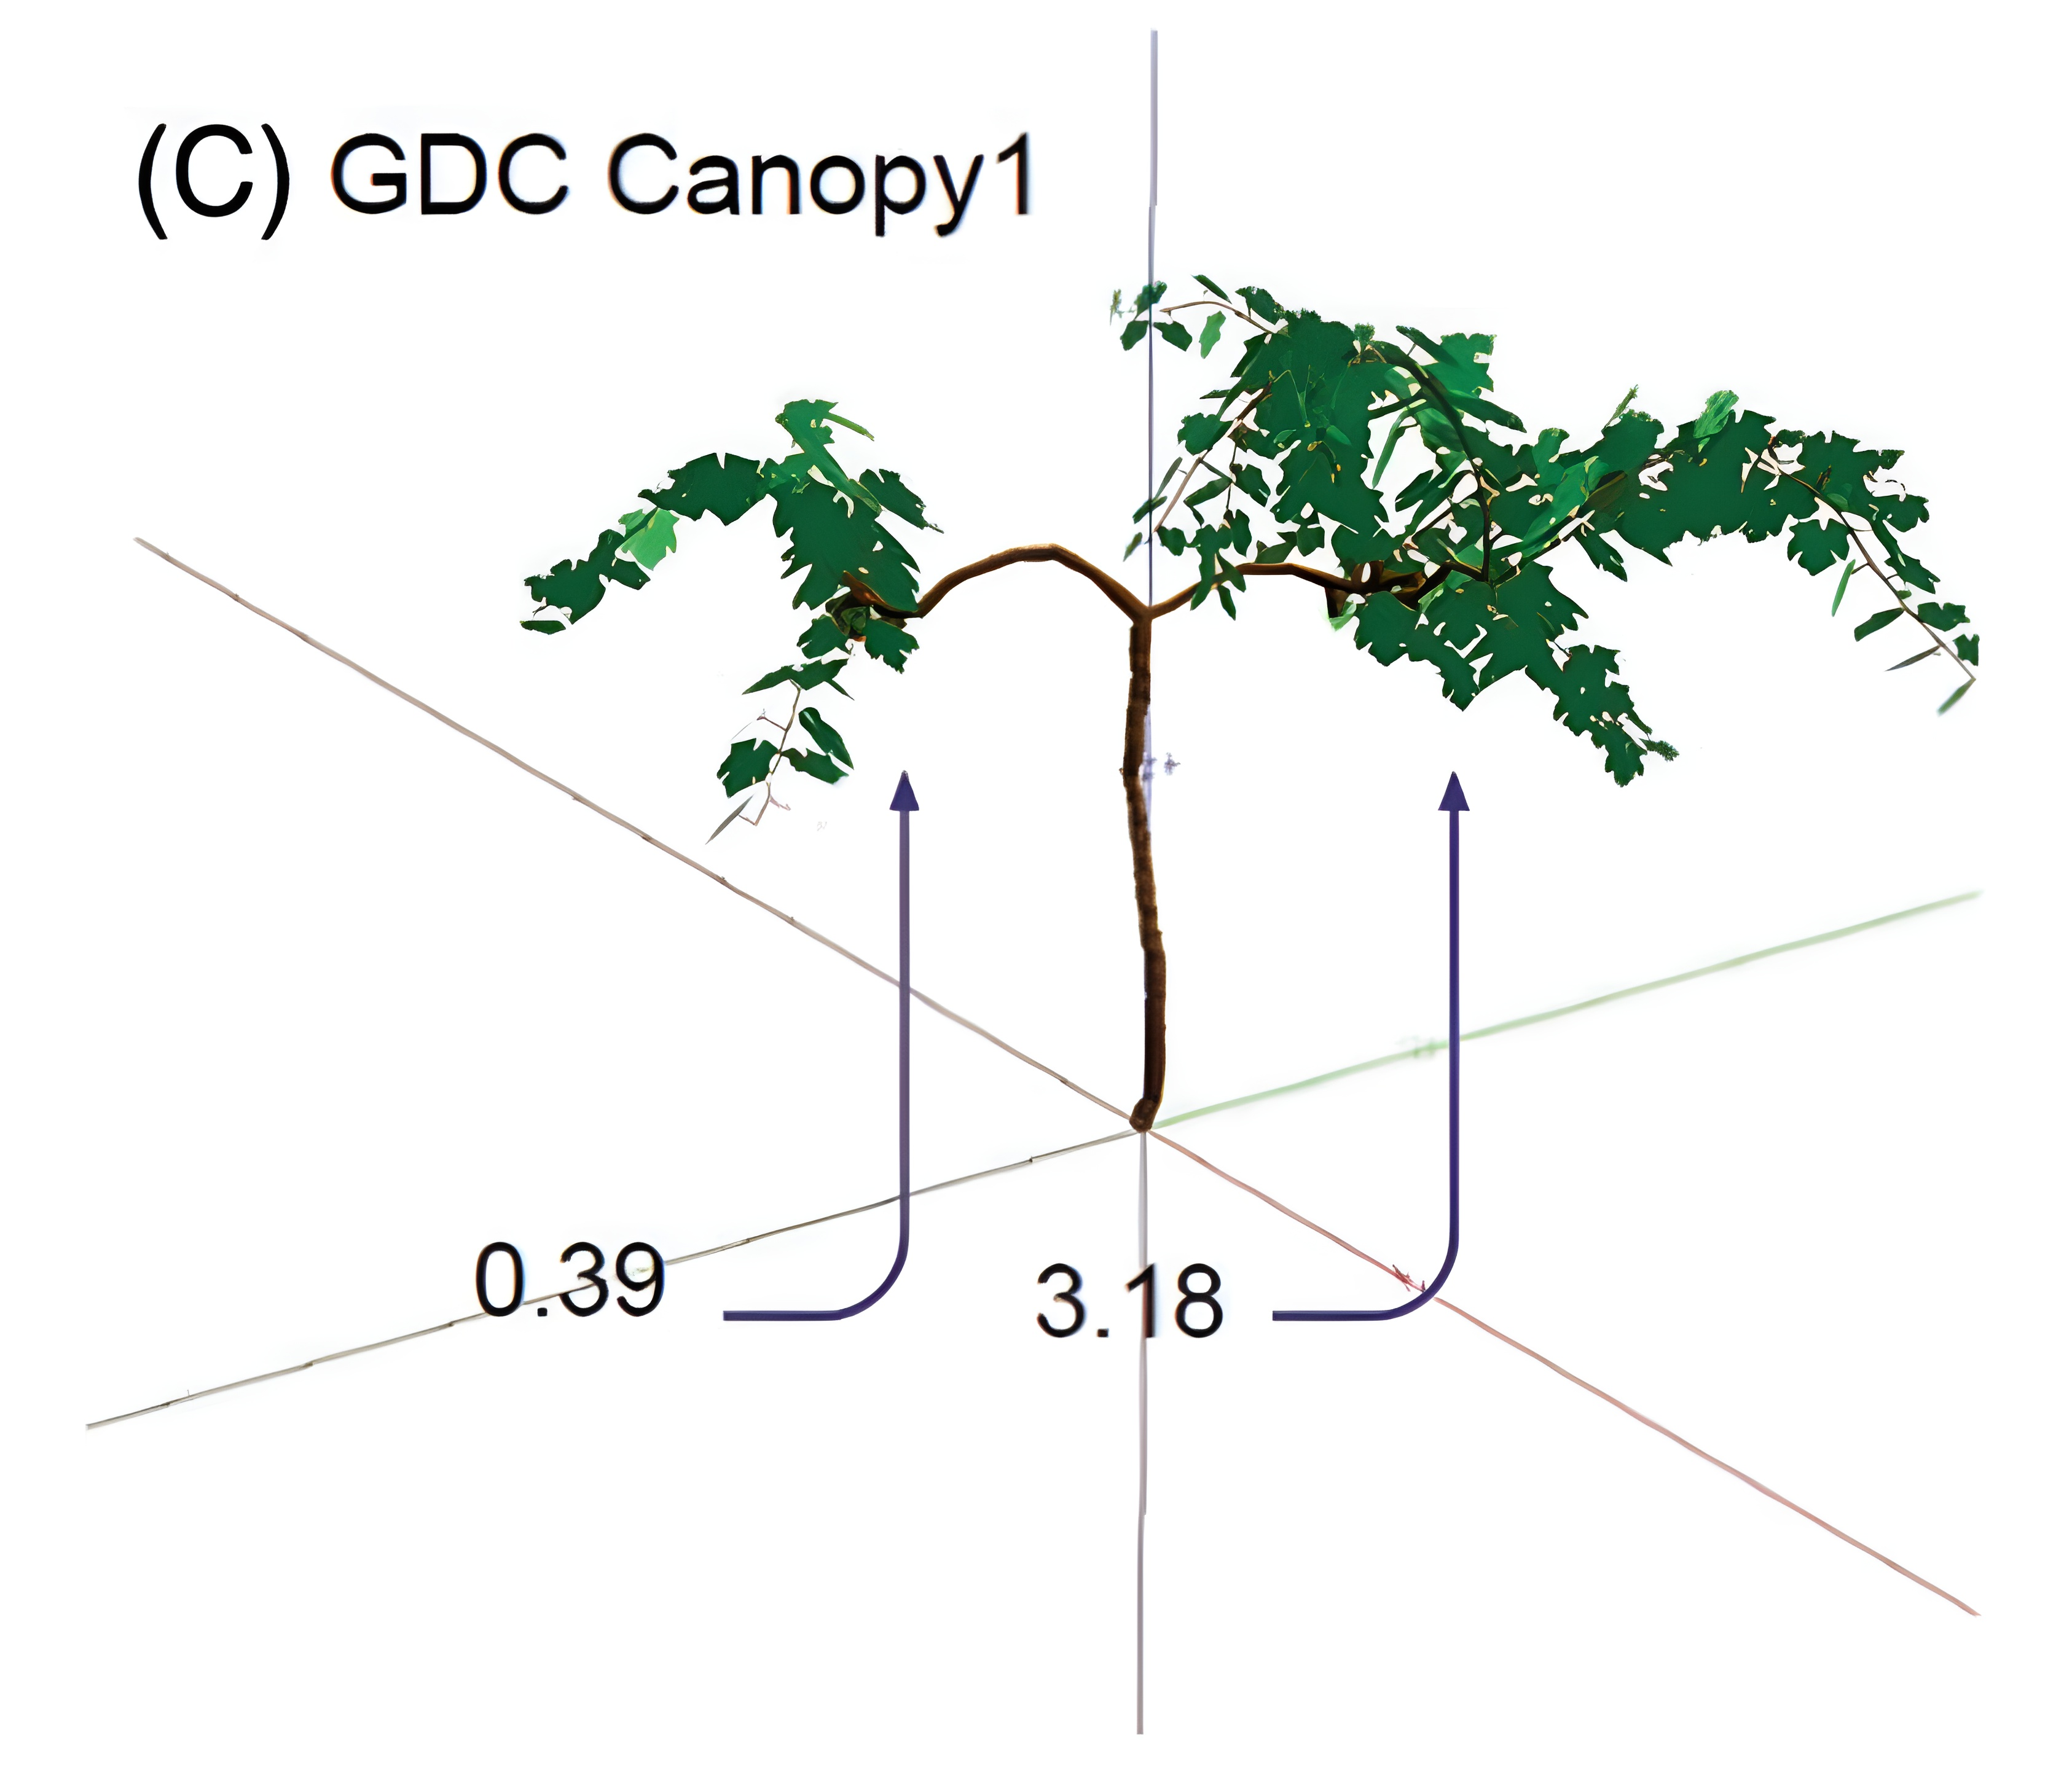
\includegraphics[width=\linewidth,height=\linewidth,keepaspectratio]{img/hydroshoot_can1_upscaled.jpg}
        \caption{HydroShoot}
        \label{fig:hydroshoot-archi}
    \end{subfigure}
    \hfill
    \begin{subfigure}[b]{0.485\linewidth}
        \centering
        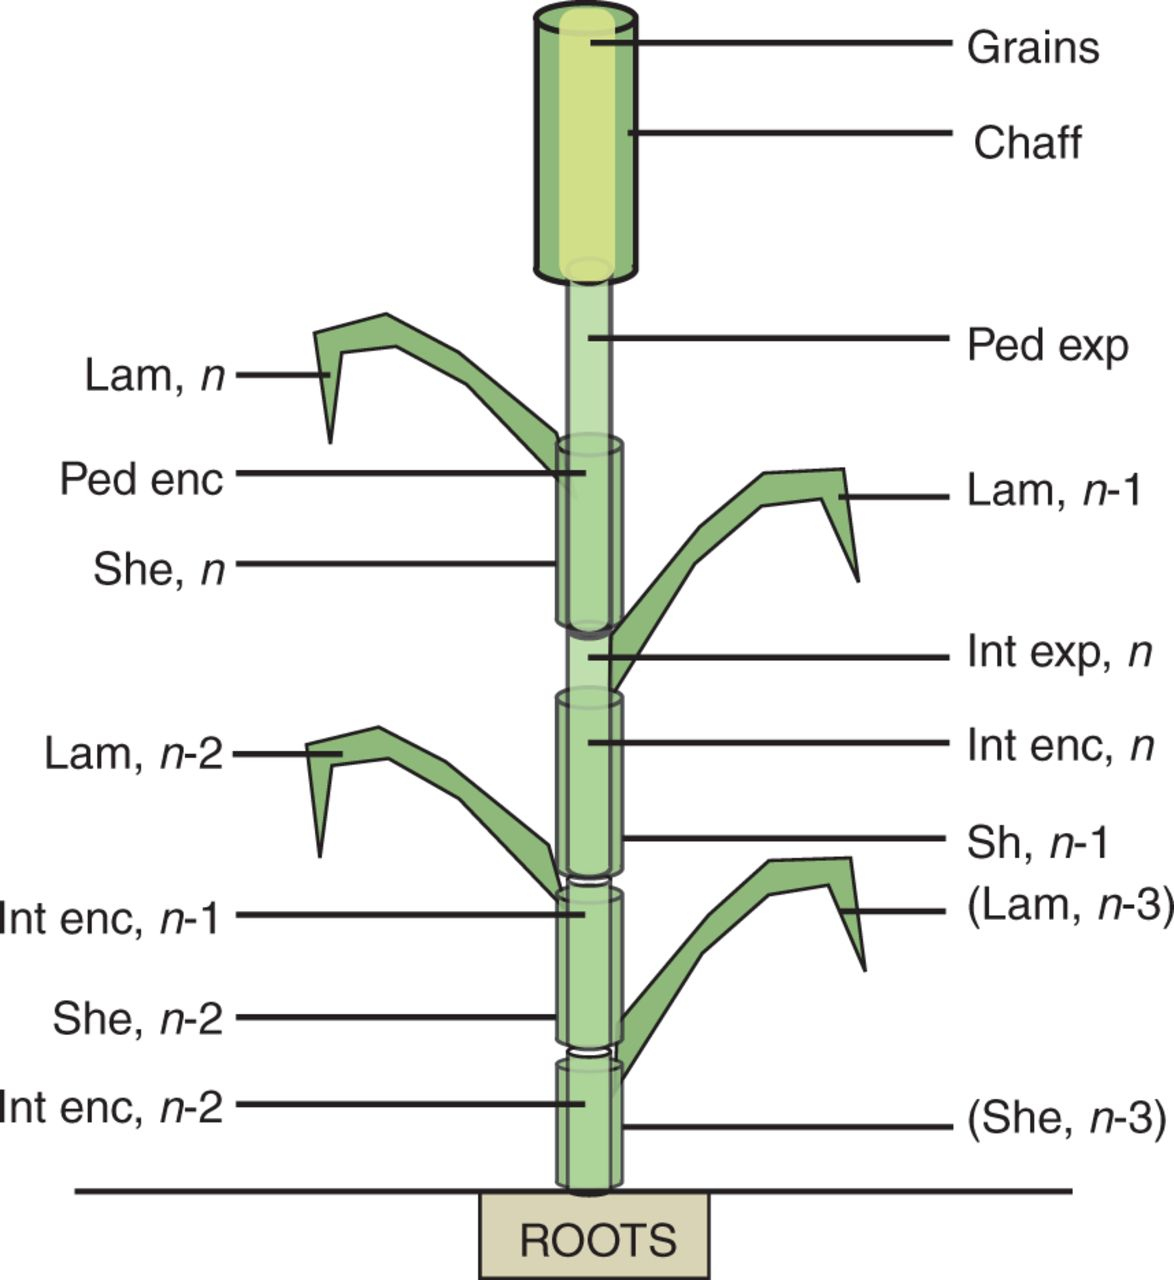
\includegraphics[width=\linewidth,height=0.85\linewidth,keepaspectratio]{img/cnwheat_architecture.jpeg}
        \caption{CN-Wheat}
        \label{fig:cnwheat-archi}
    \end{subfigure}
    \caption[FSPMs selected for use in experiments in this work.]{
            FSPMs selected for use in experiments in this work. 
            (\subref{fig:hydroshoot-archi}) A grapevine specimen from HydroShoot with the canopy trained in the ``Geneva Double Curtain'' configuration.  This figure is reused from \citet{albasha_hydroshoot_2019} under the CC BY 4.0 license.
            (\subref{fig:cnwheat-archi}) The architecture of the CN-Wheat model. This figure is reused from \citet{barillot_cn-wheat_2016} with permission from the publisher (Copyright 2016 Oxford University Press).
    }
    \label{fig:fading_memory_experiments}
\end{figure}

% CC BY 4.0 license

\subsection{Simulation Details}

Table \ref{table:simulation_details} compares the simulation details of both \acrshort{fspm}s.
HydroShoot's simulation length is relatively short, so the simulation must be run multiple times using different meteorological inputs to generate a large enough dataset.
Because of HydroShoot's large size, we will limit our observations to a small selection of leaf elements.
While CN-Wheat only has fifteen elements, we must use an even smaller subset as the reservoir because some physiological targets are a linear function of the elements. 



\begin{table}[!ht]
    \raggedright
    \caption{Comparison of HydroShoot and CN-Wheat: simulation details.}
    \label{table:simulation_details}
    \def\arraystretch{1.2}
    \begin{tabularx}{\textwidth}{
        >{\raggedright\arraybackslash} X
        >{\centering\arraybackslash} X
        >{\centering\arraybackslash} X
    }
        \toprule
        \textbf{} & \textbf{HydroShoot} & \textbf{CN-Wheat} \\ 
        \midrule
        \textbf{Simulation step} & \SI{1}{h} & \SI{1}{h} \\
        \arrayrulecolor{black!10!white}
        \midrule
        \textbf{Simulation duration} & 7 days & 50 days \\
        \midrule
        \textbf{Model structure} & static (idealized reservoir) & Post-vegetative growth \\
        \midrule
        \textbf{Model size} &  $\approx 10^3$ elements & 15 elements \\
        \arrayrulecolor{black}
        \bottomrule
    \end{tabularx}
\end{table}







\subsection{Environmental Inputs}

The environmental inputs of both models are listed in Table \ref{table:simulation_inputs}.
Significant abiotic factors are present in both models: air temperature, relative air humidity, wind speed and incident sunlight.
CO$_2$ concentration and atmospheric pressure are model inputs but use constant values during simulation. 
The available wind speed data for CN-Wheat varies daily instead of hourly, making it unsuited as a regression target or input to computational benchmarks.

% \begin{table}[!ht]
    \raggedright
    \caption{Comparison of HydroShoot and CN-Wheat: environmental models.}
    \label{table:simulation_inputs}
    \def\arraystretch{1.2}
    \begin{tabularx}{\textwidth}{
        >{\centering\arraybackslash} c
        >{\raggedright\arraybackslash} X
        >{\centering\arraybackslash} c
        >{\centering\arraybackslash} c
        >{\centering\arraybackslash} c
    }
        \toprule
        \textbf{Symbol} & \textbf{Description} & \textbf{Unit} & \textbf{HydroShoot} & \textbf{CN-Wheat} \\ 
        \midrule
        \(T_{\text{air}}\) & Air temperature & \unit{\celsius} & Hourly & Hourly \\
        \arrayrulecolor{black!10!white}
        \midrule
        \(\text{RH}\) & Relative humidity & \unit{\percent} & Hourly & Hourly \\
        \midrule
        \(u\) & Wind speed & \unit{\meter\per\second} & Hourly & Daily \\
        \midrule
        \multirow{2}{*}{\(\text{PAR}\)} & \multirow{2}{*}{\acrlong{par}} & \unit{\watt\per\meter\squared} & Hourly & / \\
        % \midrule
        & & \unit{\micro\mole\of{photons}\per\square\metre\per\second} & / & Hourly  \\
        \midrule
        CO\textsubscript{2} & CO\textsubscript{2} concentration & \unit{\micro\mole\of{CO\textsubscript{2}}\per\mol} & \SI{400}{ppm} & \SI{360}{ppm} \\
        \midrule
        \(P_a\) & Atmospheric pressure & \unit{\kilo\pascal} & \SI{101.3}{\kilo\pascal} & / \\
        \arrayrulecolor{black}
        \bottomrule
    \end{tabularx}
\end{table}

% \multirow{6}{6cm}{thermal camera}

% \begin{table}[!ht]
%     \raggedright
%     \caption{Comparison of HydroShoot and CN-Wheat: environmental models.}
%     \label{table:simulation_inputs}
%     \def\arraystretch{1.2}
%     \begin{tabularx}{\textwidth}{
%         >{\centering\arraybackslash} c
%         >{\raggedright\arraybackslash} X
%         >{\centering\arraybackslash} c
%         >{\centering\arraybackslash} c
%         >{\centering\arraybackslash} c
%     }
%         \toprule
%         \textbf{Symbol} & \textbf{Description} & \textbf{Unit} & \textbf{HydroShoot} & \textbf{CN-Wheat} \\ 
%         \midrule
%         \(T_{\text{air}}\) & Air temperature & \unit{\celsius} & Hourly & Hourly \\
%         \arrayrulecolor{black!10!white}
%         \midrule
%         \(\text{RH}\) & Relative humidity & \unit{\percent} & Hourly & Hourly \\
%         \midrule
%         \(u\) & Wind speed & \unit{\meter\per\second} & Hourly & Daily \\
%         \midrule
%         \(R_g\) & Shortwave irradiance & \unit{\watt\per\meter\squared} & Hourly & / \\
%         \midrule
%         \(I_{\text{PAR}}\) & \acrlong{par} & \unit{\micro\mole\of{photons}\per\square\metre\per\second} & / & Hourly  \\
%         \midrule
%         CO\textsubscript{2} & CO\textsubscript{2} concentration & \unit{\micro\mole\of{CO\textsubscript{2}}\per\mol} & \SI{400}{ppm} & \SI{360}{ppm} \\
%         \midrule
%         \(P_a\) & Atmospheric pressure & \unit{\kilo\pascal} & \SI{101.3}{\kilo\pascal} & / \\
%         \arrayrulecolor{black}
%         \bottomrule
%     \end{tabularx}
% \end{table}

\subsection{Regression Targets}

Table \ref{table:simulation_regression_tasks} lists the physiological regression targets that can be used for each model. 
To create more overlap between the two models, it is possible to calculate some targets not present in CN-Wheat from the observed structural elements.

% 
\begin{table}[!ht]
    \raggedright
    \caption[Comparison of HydroShoot and CN-Wheat: available regression tasks.]{Comparison of HydroShoot and CN-Wheat: available regression tasks. Check marks indicate whether the target is computed by the FSPM. Targets annotated with $\ast$ are not calculated in the simulation, but can be computed from other simulation outputs.}
    \label{table:simulation_regression_tasks}
    \def\arraystretch{1.2}
    \begin{tabularx}{\textwidth}{
        >{\centering\arraybackslash} c
        >{\raggedright\arraybackslash} X
        >{\centering\arraybackslash} c
        >{\centering\arraybackslash} c
        >{\centering\arraybackslash} c
    }
        \toprule
        \textbf{Symbol} & \textbf{Description} & \textbf{Unit} & \textbf{HydroShoot} & \textbf{CN-Wheat} \\ 
        \midrule
        \arrayrulecolor{black!10!white}
        \(E\) & Transpiration rate rate & \unit{\gram\per\hour} & \checkmark & \checkmark \\
        \midrule
        \(A_n\) & Net photosynthesis rate & \unit{\micro\mol\per\s} & \checkmark &  \\
        \midrule
        \(T_{\text{leaf}}\) & Mean leaf temperature & \unit{\celsius} & \checkmark & $\ast$ \\
        \midrule
        \multirow{2}{*}{\(\Phi_{\text{PAR}}\)} & \multirow{2}{*}{Absorbed \acrshort{par}} & \unit{\watt\per\meter\squared} & \checkmark &  \\
        % \midrule
        & & \unit{\micro\mol\per\s} & & $\ast$ \\
        \midrule
        \(R_{\text{shoot}}\) & Shoot respiration & \unit{\micro\mol\of{C}\per\second} & & \checkmark  \\
        \midrule
        \(R_{\text{roots}}\) & Root respiration & \unit{\micro\mol\of{C}\per\second} &  & \checkmark  \\
        \arrayrulecolor{black}
        \bottomrule
    \end{tabularx}
\end{table}

% \multirow{6}{6cm}{thermal camera}


% \begin{table}[!ht]
%     \raggedright
%     \caption{Comparison of HydroShoot and CN-Wheat: available regression tasks. Targets annotated with $\ast$ are not calculated in the simulation, but can be computed from other simulation outputs.}
%     \label{table:simulation_regression_tasks}
%     \def\arraystretch{1.2}
%     \begin{tabularx}{\textwidth}{
%         >{\centering\arraybackslash} c
%         >{\raggedright\arraybackslash} X
%         >{\centering\arraybackslash} c
%         >{\centering\arraybackslash} c
%         >{\centering\arraybackslash} c
%     }
%         \toprule
%         \textbf{Symbol} & \textbf{Description} & \textbf{Unit} & \textbf{HydroShoot} & \textbf{CN-Wheat} \\ 
%         \midrule
%         \arrayrulecolor{black!10!white}
%         \(E\) & Transpiration rate rate & \unit{\gram\per\hour} & \checkmark & \checkmark \\
%         \midrule
%         \(A_n\) & Net photosynthesis rate & \unit{\micro\mol\per\s} & \checkmark &  \\
%         \midrule
%         \(T_{\text{leaf}}\) & Mean leaf temperature & \unit{\celsius} & \checkmark & $\ast$ \\
%         \midrule
%         \(\Phi_{R_g}\) & Absorbed solar irradiance & \unit{\watt\per\meter\squared} & \checkmark &  \\
%         \midrule
%         \(\Phi_{I_\text{PAR}}\) & Absorbed \acrshort{par} & \unit{\micro\mol\per\s} & & $\ast$ \\
%         \midrule
%         \(R_{\text{shoot}}\) & Shoot respiration & \unit{??} & & \checkmark  \\
%         \midrule
%         \(R_{\text{roots}}\) & Root respiration & \unit{??} &  & \checkmark  \\
%         \arrayrulecolor{black}
%         \bottomrule
%     \end{tabularx}
% \end{table}

\subsection{Available Reservoirs}

The observable physiological processes for HydroShoot and CN-Wheat are presented in Table \ref{table:simulation_reservoirs}.
We limited the table to processes that would be experimentally observable, as listed in Tables \ref{table:imaging-techniques} and \ref{table:non-imaging-techniques}. 
Both models track the photosynthesis rate, surface temperature, transpiration rate, and stomatal conductance. 
HydroShoot has some additional hydraulic processes available.

% 
\begin{table}[!ht]
    \raggedright
    \caption[Comparison of HydroShoot and CN-Wheat: physiological processes observable in each structural element.]{Comparison of HydroShoot and CN-Wheat: physiological processes observable in each structural element. Not all are shown in the table; we only present the processes that are experimentally observable and that do not violate \acrshort{rc} assumptions in an obvious way. Check marks indicate whether the physiological process is modeled by the FSPM.}
    \label{table:simulation_reservoirs}
    \def\arraystretch{1.2}
    \begin{tabularx}{\textwidth}{
        >{\centering\arraybackslash} c
        >{\raggedright\arraybackslash} X
        >{\centering\arraybackslash} c
        >{\centering\arraybackslash} c
        >{\centering\arraybackslash} c
    }
        \toprule
        \textbf{Symbol} & \textbf{Description} & \textbf{Unit} & \textbf{HydroShoot} & \textbf{CN-Wheat} \\ 
        \midrule
        \(A_n\) & Net photosynthesis rate & \unit{\micro\mol\per\meter\squared\per\second} & \checkmark & \checkmark \\
        \arrayrulecolor{black!10!white}
        \midrule
        \(T_s\) & Surface temperature & \unit{\celsius} & \checkmark & \checkmark \\
        \midrule
        \(g_s\) & Stomatal conductance & \unit{\mol\per\meter\squared\per\second} & \checkmark & \checkmark \\
        \midrule
        \(E\) & Transpiration rate & \unit{\mol\of{H\textsubscript{2}O}\per\meter\squared\per\second} & \checkmark & \checkmark \\
        \midrule
        \(F\) & Water flow across segment & \unit{\kilo\gram\per\second} & \checkmark &  \\
        \midrule
        \(\Psi\) & Mean water potential of segment & \unit{\mega\pascal} & \checkmark &  \\
        \arrayrulecolor{black}
        \bottomrule
    \end{tabularx}
\end{table}

      
      

\section{Summary}

First, we formalized the selection criteria to choose which plant models are suited for our research.
We based these criteria on considerations from an \acrshort{rc}, a plant-physiological, and a practical perspective.
Next, we held a brief discussion of each \acrshort{fspm} we considered from the literature.
Then, we made a final selection of two models: HydroShoot and CN-Wheat.
We introduced the background of each model and gave its implementation details.
Finally, we summarized their properties relevant to our experiments: the environmental inputs, the available regression targets, and the observations that can be used as a reservoir.


\begin{table}[!ht]
    \raggedright
    \caption{Comparison of HydroShoot and CN-Wheat: environmental models.}
    \label{table:simulation_inputs}
    \def\arraystretch{1.2}
    \begin{tabularx}{\textwidth}{
        >{\centering\arraybackslash} c
        >{\raggedright\arraybackslash} X
        >{\centering\arraybackslash} c
        >{\centering\arraybackslash} c
        >{\centering\arraybackslash} c
    }
        \toprule
        \textbf{Symbol} & \textbf{Description} & \textbf{Unit} & \textbf{HydroShoot} & \textbf{CN-Wheat} \\ 
        \midrule
        \(T_{\text{air}}\) & Air temperature & \unit{\celsius} & Hourly & Hourly \\
        \arrayrulecolor{black!10!white}
        \midrule
        \(\text{RH}\) & Relative humidity & \unit{\percent} & Hourly & Hourly \\
        \midrule
        \(u\) & Wind speed & \unit{\meter\per\second} & Hourly & Daily \\
        \midrule
        \multirow{2}{*}{\(\text{PAR}\)} & \multirow{2}{*}{\acrlong{par}} & \unit{\watt\per\meter\squared} & Hourly & / \\
        % \midrule
        & & \unit{\micro\mole\of{photons}\per\square\metre\per\second} & / & Hourly  \\
        \midrule
        CO\textsubscript{2} & CO\textsubscript{2} concentration & \unit{\micro\mole\of{CO\textsubscript{2}}\per\mol} & \SI{400}{ppm} & \SI{360}{ppm} \\
        \midrule
        \(P_a\) & Atmospheric pressure & \unit{\kilo\pascal} & \SI{101.3}{\kilo\pascal} & / \\
        \arrayrulecolor{black}
        \bottomrule
    \end{tabularx}
\end{table}

% \multirow{6}{6cm}{thermal camera}

% \begin{table}[!ht]
%     \raggedright
%     \caption{Comparison of HydroShoot and CN-Wheat: environmental models.}
%     \label{table:simulation_inputs}
%     \def\arraystretch{1.2}
%     \begin{tabularx}{\textwidth}{
%         >{\centering\arraybackslash} c
%         >{\raggedright\arraybackslash} X
%         >{\centering\arraybackslash} c
%         >{\centering\arraybackslash} c
%         >{\centering\arraybackslash} c
%     }
%         \toprule
%         \textbf{Symbol} & \textbf{Description} & \textbf{Unit} & \textbf{HydroShoot} & \textbf{CN-Wheat} \\ 
%         \midrule
%         \(T_{\text{air}}\) & Air temperature & \unit{\celsius} & Hourly & Hourly \\
%         \arrayrulecolor{black!10!white}
%         \midrule
%         \(\text{RH}\) & Relative humidity & \unit{\percent} & Hourly & Hourly \\
%         \midrule
%         \(u\) & Wind speed & \unit{\meter\per\second} & Hourly & Daily \\
%         \midrule
%         \(R_g\) & Shortwave irradiance & \unit{\watt\per\meter\squared} & Hourly & / \\
%         \midrule
%         \(I_{\text{PAR}}\) & \acrlong{par} & \unit{\micro\mole\of{photons}\per\square\metre\per\second} & / & Hourly  \\
%         \midrule
%         CO\textsubscript{2} & CO\textsubscript{2} concentration & \unit{\micro\mole\of{CO\textsubscript{2}}\per\mol} & \SI{400}{ppm} & \SI{360}{ppm} \\
%         \midrule
%         \(P_a\) & Atmospheric pressure & \unit{\kilo\pascal} & \SI{101.3}{\kilo\pascal} & / \\
%         \arrayrulecolor{black}
%         \bottomrule
%     \end{tabularx}
% \end{table}

\begin{table}[!ht]
    \raggedright
    \caption[Comparison of HydroShoot and CN-Wheat: available regression tasks.]{Comparison of HydroShoot and CN-Wheat: available regression tasks. Check marks indicate whether the target is computed by the FSPM. Targets annotated with $\ast$ are not calculated in the simulation, but can be computed from other simulation outputs.}
    \label{table:simulation_regression_tasks}
    \def\arraystretch{1.2}
    \begin{tabularx}{\textwidth}{
        >{\centering\arraybackslash} c
        >{\raggedright\arraybackslash} X
        >{\centering\arraybackslash} c
        >{\centering\arraybackslash} c
        >{\centering\arraybackslash} c
    }
        \toprule
        \textbf{Symbol} & \textbf{Description} & \textbf{Unit} & \textbf{HydroShoot} & \textbf{CN-Wheat} \\ 
        \midrule
        \arrayrulecolor{black!10!white}
        \(E\) & Transpiration rate rate & \unit{\gram\per\hour} & \checkmark & \checkmark \\
        \midrule
        \(A_n\) & Net photosynthesis rate & \unit{\micro\mol\per\s} & \checkmark &  \\
        \midrule
        \(T_{\text{leaf}}\) & Mean leaf temperature & \unit{\celsius} & \checkmark & $\ast$ \\
        \midrule
        \multirow{2}{*}{\(\Phi_{\text{PAR}}\)} & \multirow{2}{*}{Absorbed \acrshort{par}} & \unit{\watt\per\meter\squared} & \checkmark &  \\
        % \midrule
        & & \unit{\micro\mol\per\s} & & $\ast$ \\
        \midrule
        \(R_{\text{shoot}}\) & Shoot respiration & \unit{\micro\mol\of{C}\per\second} & & \checkmark  \\
        \midrule
        \(R_{\text{roots}}\) & Root respiration & \unit{\micro\mol\of{C}\per\second} &  & \checkmark  \\
        \arrayrulecolor{black}
        \bottomrule
    \end{tabularx}
\end{table}

% \multirow{6}{6cm}{thermal camera}


% \begin{table}[!ht]
%     \raggedright
%     \caption{Comparison of HydroShoot and CN-Wheat: available regression tasks. Targets annotated with $\ast$ are not calculated in the simulation, but can be computed from other simulation outputs.}
%     \label{table:simulation_regression_tasks}
%     \def\arraystretch{1.2}
%     \begin{tabularx}{\textwidth}{
%         >{\centering\arraybackslash} c
%         >{\raggedright\arraybackslash} X
%         >{\centering\arraybackslash} c
%         >{\centering\arraybackslash} c
%         >{\centering\arraybackslash} c
%     }
%         \toprule
%         \textbf{Symbol} & \textbf{Description} & \textbf{Unit} & \textbf{HydroShoot} & \textbf{CN-Wheat} \\ 
%         \midrule
%         \arrayrulecolor{black!10!white}
%         \(E\) & Transpiration rate rate & \unit{\gram\per\hour} & \checkmark & \checkmark \\
%         \midrule
%         \(A_n\) & Net photosynthesis rate & \unit{\micro\mol\per\s} & \checkmark &  \\
%         \midrule
%         \(T_{\text{leaf}}\) & Mean leaf temperature & \unit{\celsius} & \checkmark & $\ast$ \\
%         \midrule
%         \(\Phi_{R_g}\) & Absorbed solar irradiance & \unit{\watt\per\meter\squared} & \checkmark &  \\
%         \midrule
%         \(\Phi_{I_\text{PAR}}\) & Absorbed \acrshort{par} & \unit{\micro\mol\per\s} & & $\ast$ \\
%         \midrule
%         \(R_{\text{shoot}}\) & Shoot respiration & \unit{??} & & \checkmark  \\
%         \midrule
%         \(R_{\text{roots}}\) & Root respiration & \unit{??} &  & \checkmark  \\
%         \arrayrulecolor{black}
%         \bottomrule
%     \end{tabularx}
% \end{table}

\begin{table}[!ht]
    \raggedright
    \caption[Comparison of HydroShoot and CN-Wheat: physiological processes observable in each structural element.]{Comparison of HydroShoot and CN-Wheat: physiological processes observable in each structural element. Not all are shown in the table; we only present the processes that are experimentally observable and that do not violate \acrshort{rc} assumptions in an obvious way. Check marks indicate whether the physiological process is modeled by the FSPM.}
    \label{table:simulation_reservoirs}
    \def\arraystretch{1.2}
    \begin{tabularx}{\textwidth}{
        >{\centering\arraybackslash} c
        >{\raggedright\arraybackslash} X
        >{\centering\arraybackslash} c
        >{\centering\arraybackslash} c
        >{\centering\arraybackslash} c
    }
        \toprule
        \textbf{Symbol} & \textbf{Description} & \textbf{Unit} & \textbf{HydroShoot} & \textbf{CN-Wheat} \\ 
        \midrule
        \(A_n\) & Net photosynthesis rate & \unit{\micro\mol\per\meter\squared\per\second} & \checkmark & \checkmark \\
        \arrayrulecolor{black!10!white}
        \midrule
        \(T_s\) & Surface temperature & \unit{\celsius} & \checkmark & \checkmark \\
        \midrule
        \(g_s\) & Stomatal conductance & \unit{\mol\per\meter\squared\per\second} & \checkmark & \checkmark \\
        \midrule
        \(E\) & Transpiration rate & \unit{\mol\of{H\textsubscript{2}O}\per\meter\squared\per\second} & \checkmark & \checkmark \\
        \midrule
        \(F\) & Water flow across segment & \unit{\kilo\gram\per\second} & \checkmark &  \\
        \midrule
        \(\Psi\) & Mean water potential of segment & \unit{\mega\pascal} & \checkmark &  \\
        \arrayrulecolor{black}
        \bottomrule
    \end{tabularx}
\end{table}

      
      